\documentclass[a4paper,11pt]{article}
\pdfoutput=1 % if your are submitting a pdflatex (i.e. if you have
             % images in pdf, png or jpg format)

\usepackage{jcappub} % for details on the use of the package, please
                     % see the JCAP-author-manual

\usepackage[T1]{fontenc} % if needed


%\title{\boldmath A title with some math: $x=1$}
\title{Full simulation of the Terzina telescope}


%% %simple case: 2 authors, same institution
%% \author{A. Uthor}
%% \author{and A. Nother Author}
%% \affiliation{Institution,\\Address, Country}
%% more complex case: 4 authors, 3 institutions, 2 footnotes
%\author[a,b,1]{F. Irst,\note{Corresponding author.}}
%\author[c]{S. Econd,}
%\author[a,2]{T. Hird\note{Also at Some University.}}
%\author[a,2]{and Fourth}
%% The "\note" macro will give a warning: "Ignoring empty anchor..."
%% you can safely ignore it.
%%\affiliation[a]{One University,\\some-street, Country}
%%\affiliation[b]{Another University,\\different-address, Country}
%%\affiliation[c]{A School for Advanced Studies,\\some-location, Country}
%% e-mail addresses: one for each author, in the same order as the authors
%%\emailAdd{first@one.univ}
%%\emailAdd{second@asas.edu}
%%\emailAdd{third@one.univ}
%%\emailAdd{fourth@one.univ}

%authors
\author[a]{L. Burmistrov,}

%affiliation
\affiliation[a]{University of Geneva,\\Geneva, Switzerland}

% e-mail addresses
\emailAdd{leonid.burmistrov@unige.ch}

\abstract{ Some first seed :-) ....
Terzina is a satellite base Cherenkov telescope designed to operate at $\sim$535~km altitude with sun-synchronous orbit. Its primary goal is to probe the new concept of detecting ultra high energy cosmic rays and neutrinos by observing Cherenkov light from an extensive shower produced in the atmosphere. It is part of the NUSES space mission with a wide scientific program. Also, the mission includes the ZIR\`E apparatus for flux measurements of electrons, protons, light nuclei with energies spanning from a few to hundreds of MeV's and MeV gamma rays.

The telescope is composed of a spherical primary mirror, a small spherical mirror, a corrector lens, and Photon detection plane. The optical system can fit the tube-like envelope with 394~mm diameter and 350~mm length. It is inclined by $67.5^{\mathrm{o}}$ with respect to nadir, having an optical axis pointing towards the Earth limb. The photon detector plane is conceived to detect the photons from below and above the limb. It has a rectangular shape with a $2\times5$ aspect ratio. The camera is composed of 10 SiPM arrays ($8~\times~8$) pixel each and $3~\times~3$~mm$^{2}$ pixel size. The telescope have $7^{\mathrm{o}}$ Field-of-View this corresponds to $0.18^{\mathrm{o}}$ per pixel. It can observe the vast volume of the atmosphere with $140~\times~360$~km in cos-section.

To estimate expected signal we develop full Geant4 based simulation of the Terzina telescope. It takes into account mirror and corrector lens reflectivity and transparency, quantum efficiency and geometry of the photon sensitive camera. We use Emission for Extensive Air Showers Cherenkov Simulation (EASCherSim) as event generator.

}

\begin{document}
\maketitle
\flushbottom

\section{Intro.}
\label{sec:intro}

For internal references use label-refs: see section~\ref{sec:intro}.
Bibliographic citations can be done with cite: refs.~\cite{a,b,c}.
See figure~\ref{fig:i} and table~\ref{tab:i}.

\begin{figure}[tbp]
\centering % \begin{center}/\end{center} takes some additional vertical space
%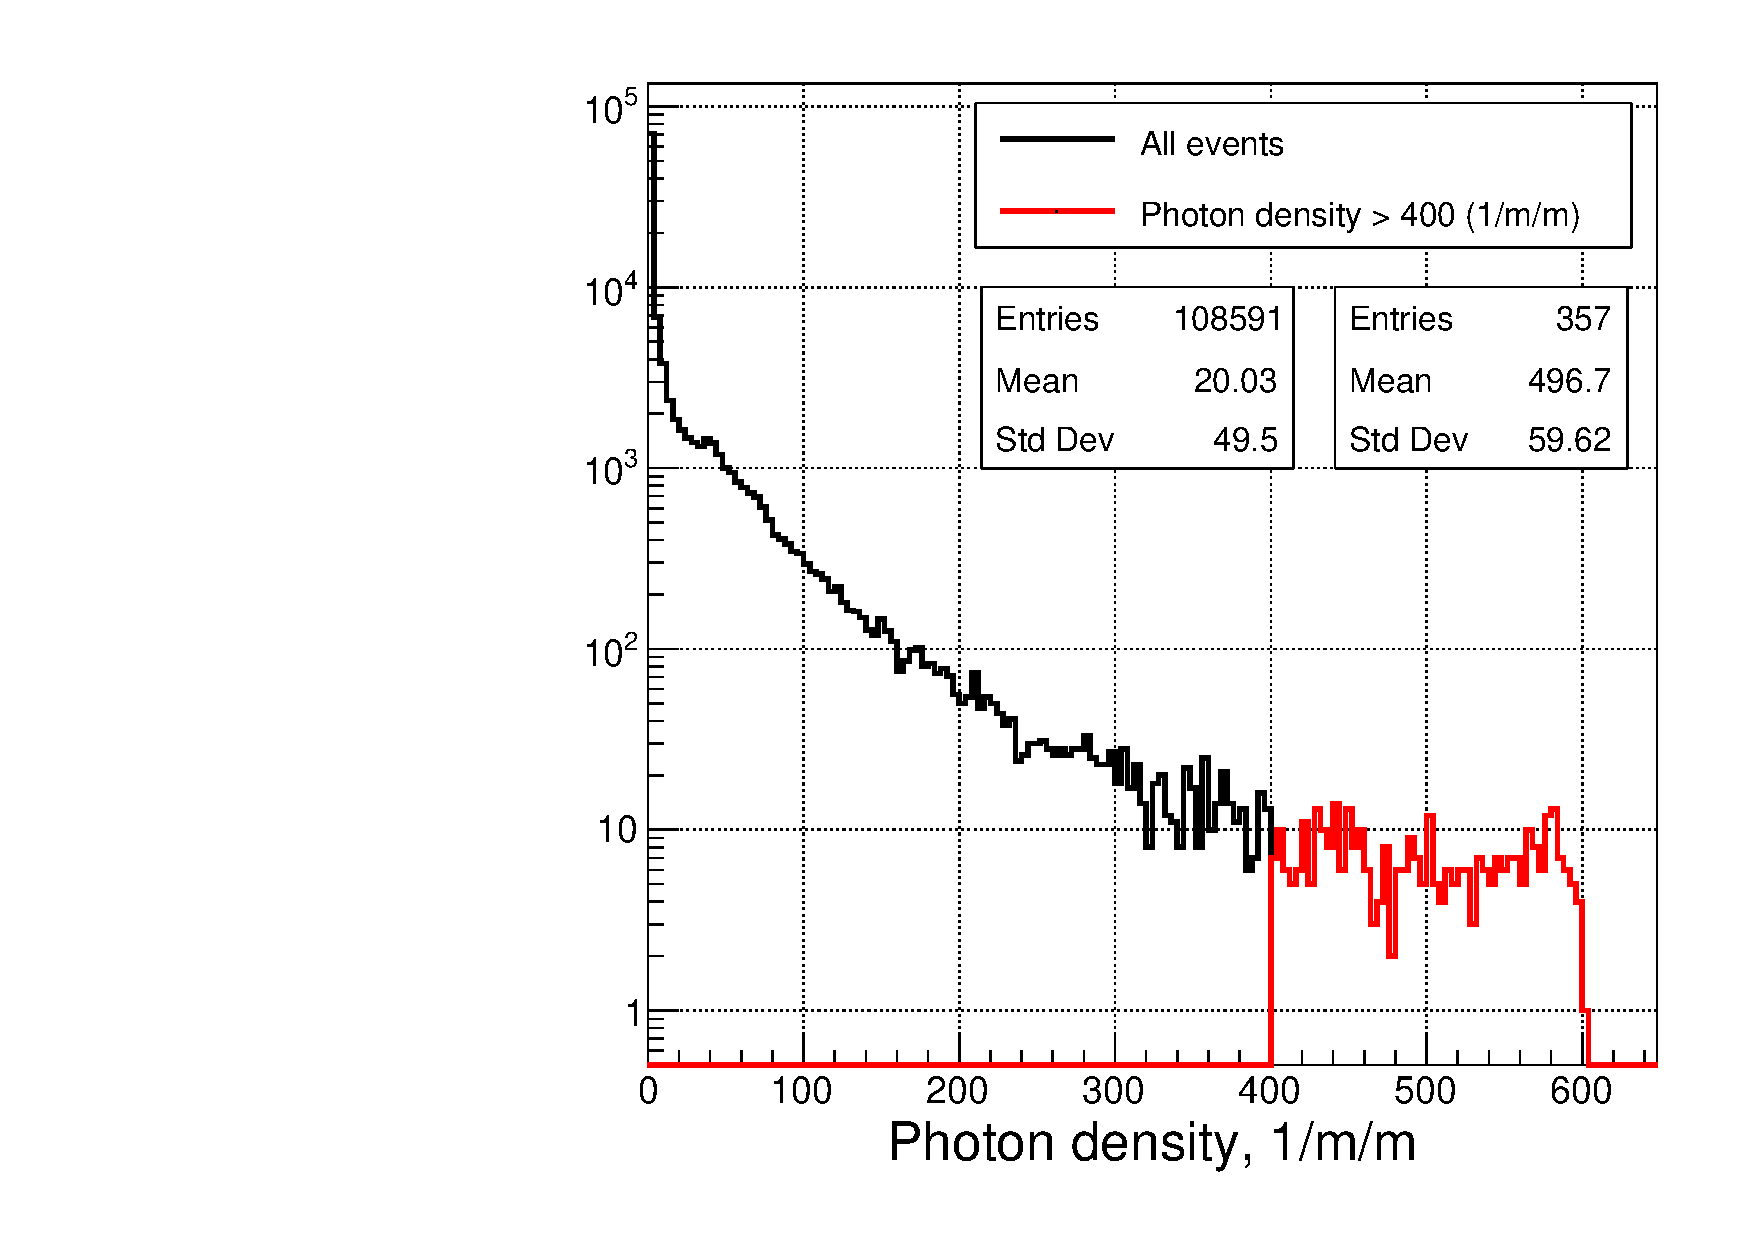
\includegraphics[width=.45\textwidth,trim=0 380 0 200,clip]{./fig_pdf/photon_density_cut.pdf}
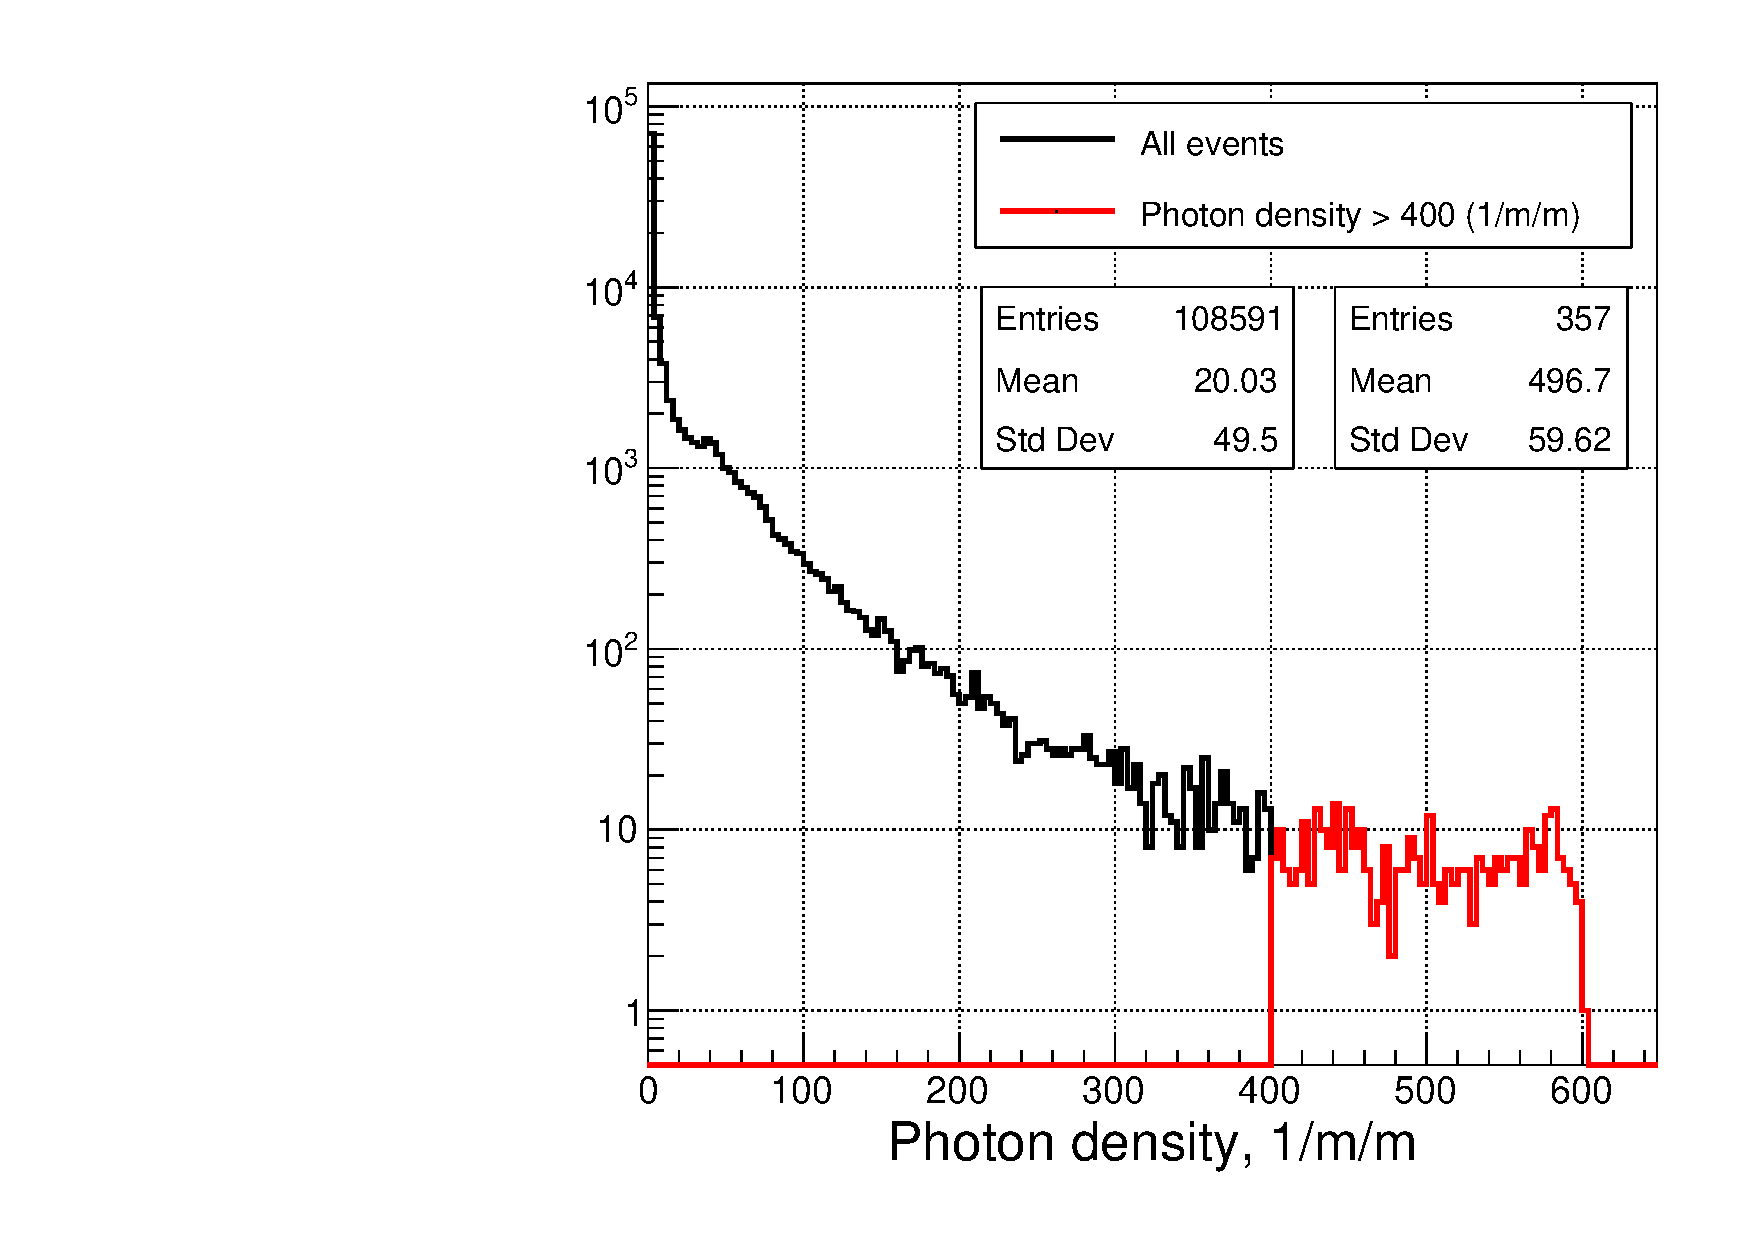
\includegraphics[width=.45\textwidth]{./fig_pdf/photon_density_cut.pdf}
\hfill
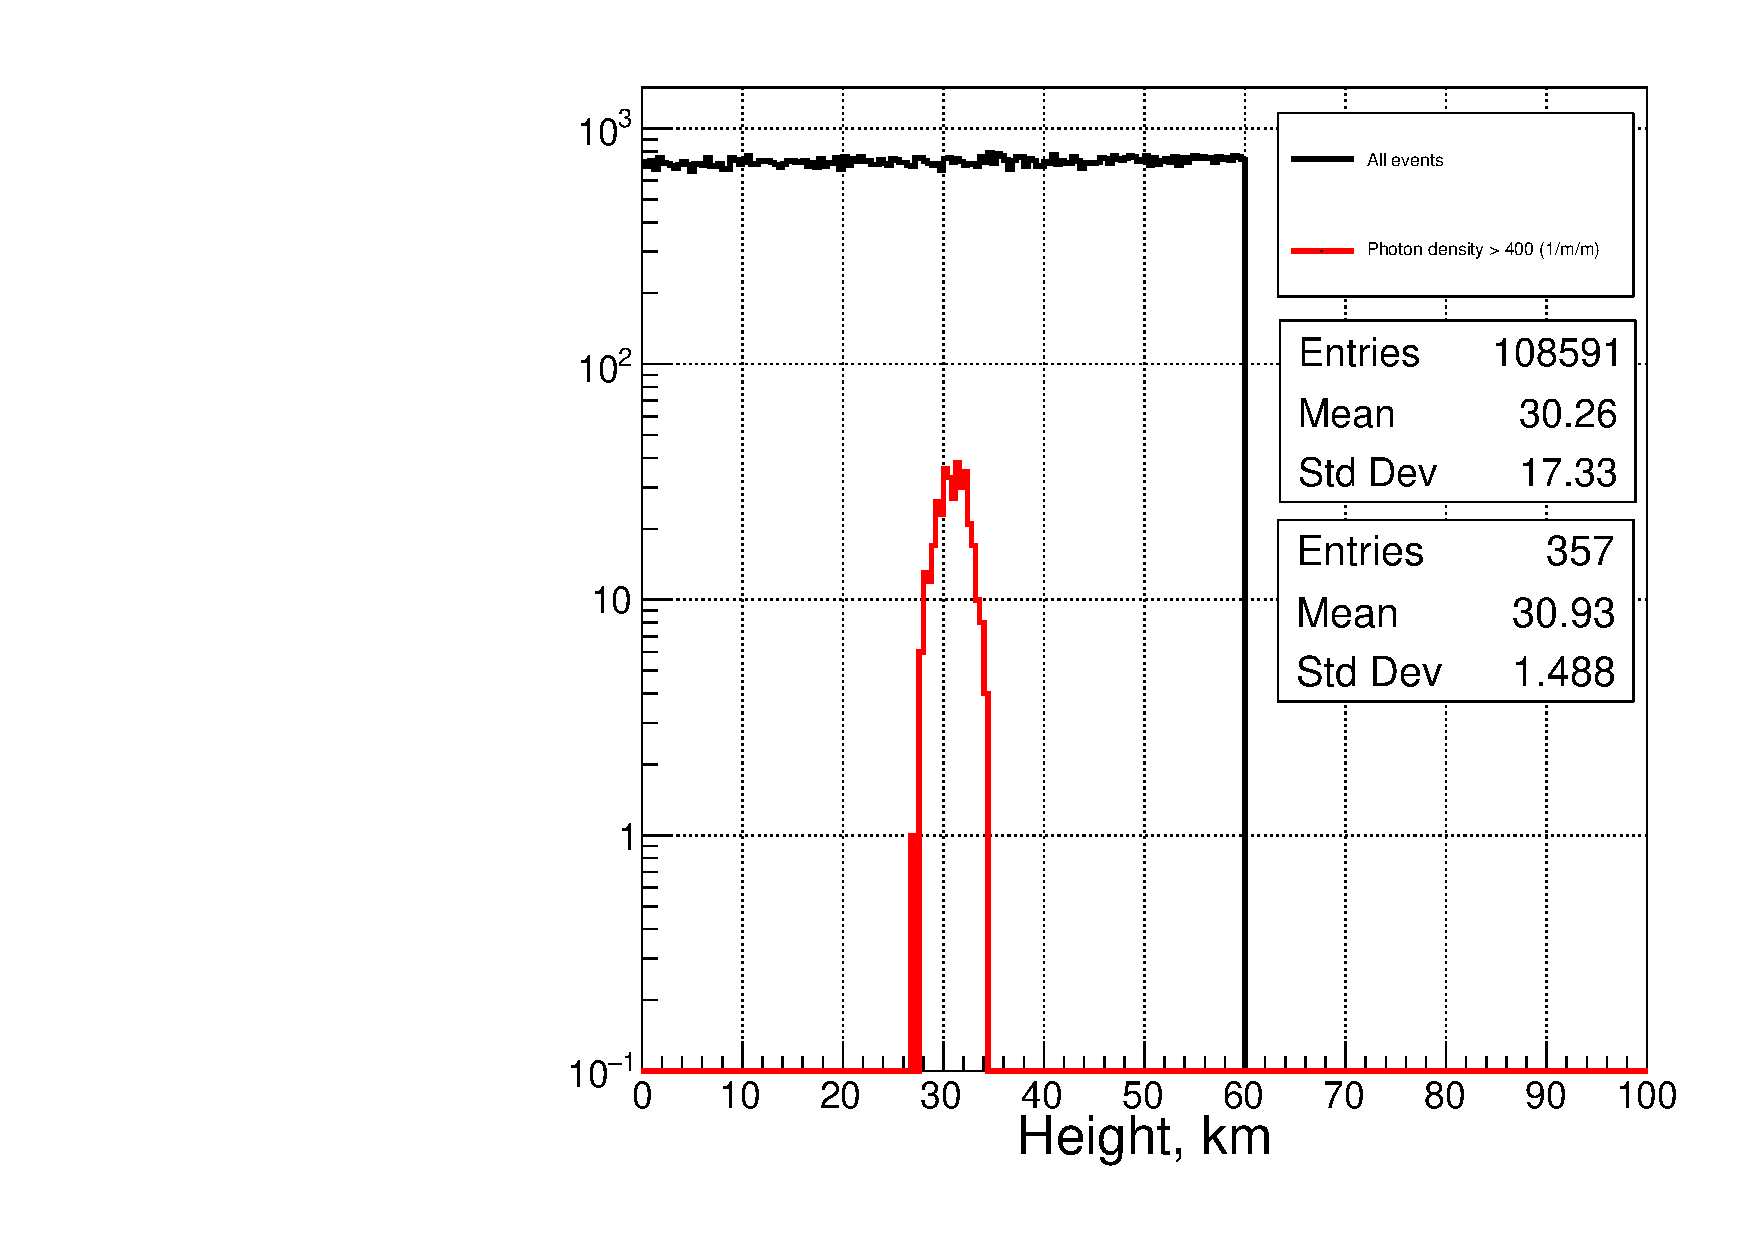
\includegraphics[width=.45\textwidth,origin=c,angle=0]{./fig_pdf/height_cut.pdf}
% "\includegraphics" is very powerful; the graphicx package is already loaded
\caption{\label{fig:i} Always give a caption.}
\end{figure}

\begin{table}[tbp]
\centering
\begin{tabular}{|lr|c|}
\hline
x&y&x and y\\
\hline
a & b & a and b\\
1 & 2 & 1 and 2\\
$\alpha$ & $\beta$ & $\alpha$ and $\beta$\\
\hline
\end{tabular}
\caption{\label{tab:i} We prefer to have borders around the tables.}
\end{table}

\section{The telescope}
\subsection{The telescope sim.}
\subsubsection{The telescope sim.}
\paragraph{Up to paragraphs.} 


\appendix
\section{Appendix}
Please always give a title also for appendices.

\acknowledgments

This is the most common positions for acknowledgments. A macro is
available to maintain the same layout and spelling of the heading.

\paragraph{Note added.} This is also a good position for notes added
after the paper has been written.



% The bibliography will probably be heavily edited during typesetting.
% We'll parse it and, using the arxiv number or the journal data, will
% query inspire, trying to verify the data (this will probalby spot
% eventual typos) and retrive the document DOI and eventual errata.
% We however suggest to always provide author, title and journal data:
% in short all the informations that clearly identify a document.

\begin{thebibliography}{99}

\bibitem{a}
Author, \emph{Title}, \emph{J. Abbrev.} {\bf vol} (year) pg.

\bibitem{b}
Author, \emph{Title},
arxiv:1234.5678.

\bibitem{c}
Author, \emph{Title},
Publisher (year).


% Please avoid comments such as "For a review'', "For some examples",
% "and references therein" or move them in the text. In general,
% please leave only references in the bibliography and move all
% accessory text in footnotes.

% Also, please have only one work for each \bibitem.


\end{thebibliography}
\end{document}
